\chapter{Cieľ práce, metodika práce a metódy skúmania}

%% ═══════════════════════════════════════════════════════════════════════════
%% 3.1  CIEĽ PRÁCE
%% ═══════════════════════════════════════════════════════════════════════════
\section{Cieľ práce}
\label{sec:ciel}

\indent Z prehľadu súčasného stavu vyplynulo, že neurónovým prístupom
k problému obchodného cestujúceho chýba spoločný metodický základ:
práce sa líšia formuláciou úlohy, kvalitou referenčných riešení aj
spôsobom hodnotenia, čo znemožňuje priame porovnanie architektúr.
Práve táto medzera motivovala zvolený prístup — grafovú formuláciu
postavenou na predikcii hrán s jednotným hodnotením na štandardných
inštanciách TSPLIB
\parencite{joshi2022generalization,bengio2021mlco,reinelt1991tsplib}.

\AssignmentGoalSK

\indent Tretiu zo stanovených úloh sme v rámci práce rozvinuli do
piatich merateľných čiastkových cieľov, ktoré pokrývajú celý postup
od prípravy údajov až po záverečnú interpretáciu výsledkov:

\begin{enumerate}
    \item Pripraviť syntetické tréningové a validačné údaje s dvoma
          úrovňami kvality referenčných riešení a spracovať štandardné
          testovacie inštancie z knižnice TSPLIB.
    \item Navrhnúť a implementovať tri rodiny modelov založených na
          predikcii hrán v úplnom grafe, od jednoduchého hranového
          perceptrónu cez reziduálny variant až po kontextový transformer.
    \item Vytvoriť jednotný hodnotiaci rámec, v ktorom sa modely aj
          heuristické bázy porovnávajú na rovnakých štrnástich inštanciách
          TSPLIB za rovnakých dekódovacích podmienok.
    \item Porovnať vplyv kvality tréningových štítkov a dekódovacích
          stratégií na výslednú kvalitu riešení.
    \item Analyzovať, či kontextový model prináša merateľné zlepšenie
          oproti lokálnym hranovým modelom, a identifikovať podmienky,
          v ktorých sú jednotlivé prístupy najefektívnejšie.
\end{enumerate}

%% ═══════════════════════════════════════════════════════════════════════════
%% 3.2  PREHĽAD EXPERIMENTÁLNEHO POSTUPU
%% ═══════════════════════════════════════════════════════════════════════════
\section{Prehľad experimentálneho postupu}
\label{sec:prehlad_postupu}

\indent Praktická časť práce bola realizovaná ako ucelený experimentálny
postup, v ktorom jednotlivé kroky priamo nadväzujú jeden na druhý. Keďže
pri dátovo riadených prístupoch ku kombinatorickej optimalizácii nemožno
oddeliť model od spôsobu prípravy dát, kvality referenčných riešení
a následného spracovania výstupu, metodická časť je koncipovaná ako opis
tohto celku, nie len jeho modelovej zložky
\parencite{bengio2021mlco,joshi2022generalization,cappart2023gnnco}.

\indent Z hľadiska údajov bol postup rozdelený na dve vzájomne prepojené
vetvy. Prvú tvorili synteticky generované euklidovské inštancie, nad
ktorými prebiehalo trénovanie a validácia modelov, pričom referenčné
riešenia sa pripravili v dvoch variantoch kvality: heuristickom
a presnom pomocou riešiča Concorde \parencite{concorde2003solver}. Druhú
vetvu tvorili štandardné inštancie z knižnice TSPLIB, ktoré slúžili
výhradne na nezávislé záverečné hodnotenie a neboli súčasťou trénovacej
množiny \parencite{reinelt1991tsplib}. Toto oddelenie umožnilo sledovať,
do akej miery sa naučené vzory prenášajú na úlohy odlišné od synteticky
generovaných príkladov.

\indent Nad oboma vetvami sa uplatnila jednotná modelová časť: všetky
inštancie sa previedli na grafovú reprezentáciu a modely sa učili
predikovať príslušnosť hrán k výslednej trase. Takáto formulácia
udržiava rovnaké experimentálne podmienky pre všetky tri porovnávané
rodiny architektúr a priamo previazuje modelový výstup s následným
dekódovaním trasy. Celkový návrh zachytáva obrázok~\ref{fig:method_overview}.

\begin{figure}[H]
    \centering
    \resizebox{0.96\textwidth}{!}{% method_overview.tex
% Vyžaduje \usetikzlibrary{arrows.meta,positioning,calc}
% Použitie: \resizebox{0.90\textwidth}{!}{% method_overview.tex
% Vyžaduje \usetikzlibrary{arrows.meta,positioning,calc}
% Použitie: \resizebox{0.90\textwidth}{!}{% method_overview.tex
% Vyžaduje \usetikzlibrary{arrows.meta,positioning,calc}
% Použitie: \resizebox{0.90\textwidth}{!}{\input{figures/tikz/method_overview}}
\begin{tikzpicture}[
    font=\small,
    node distance=0.65cm,
    header/.style={
        draw, rounded corners=4pt, align=center,
        minimum width=3.7cm, inner sep=5pt,
        font=\small\bfseries,
        text=#1!80!black, fill=#1!10, draw=#1!55
    },
    train/.style={
        draw=blue!40, fill=blue!6, rounded corners=3pt,
        align=center, minimum width=3.7cm, inner sep=5pt
    },
    refbox/.style={
        draw=orange!45, fill=orange!8, rounded corners=3pt,
        align=center, minimum width=1.72cm, inner sep=5pt
    },
    evalbox/.style={
        draw=green!50, fill=green!6, rounded corners=3pt,
        align=center, minimum width=3.7cm, inner sep=5pt
    },
    decodebox/.style={
        draw=gray!50, fill=gray!8, rounded corners=3pt,
        align=center, minimum width=5.4cm, inner sep=5pt
    },
    finalbox/.style={
        draw=gray!55, fill=gray!12, rounded corners=4pt,
        align=center, minimum width=9.8cm, inner sep=5pt
    },
    arrow/.style={
        -{Latex[length=2.6mm, width=1.9mm]}, thick,
        shorten >=3pt
    },
    darrow/.style={
        -{Latex[length=2.6mm, width=1.9mm]}, thick,
        dashed, draw=gray!60, shorten >=3pt
    },
    pline/.style={thick}
]

%% ── Uzly ──────────────────────────────────────────────────────────
\node[header=blue]  (htrain) at (0.0, 0.0) {Tréningová vetva};
\node[header=green] (heval)  at (6.8, 0.0) {Hodnotiaca vetva};

\node[train, below=of htrain] (synth)
    {Syntetické inštancie\\[2pt]\(n \in \{20,30,\ldots,100\}\)};

\node[train, below=of synth] (ref)
    {Referenčné riešenia};

%% heur a conc: väčší gap 1.40cm — dostatok priestoru pre šípky
\node[refbox, below=1.40cm of ref, xshift=-1.18cm] (heur)
    {Heuristické\\[2pt]\scriptsize(NN + 2-opt)};
\node[refbox, below=1.40cm of ref, xshift= 1.18cm] (conc)
    {Presné\\[2pt]\scriptsize(Concorde)};

%% trainmod: štandardný gap od spodku heur/conc
\node[train, below=1.20cm of heur.south |- conc.south] (trainmod)
    {Trénovanie modelov\\[2pt]MLP,\ ResMLP,\ Transformer};

\node[evalbox] at (heval |- synth)    (tsplib)
    {14 inštancií TSPLIB\\[2pt]štandardné benchmarky};
\node[evalbox] at (heval |- trainmod) (evalmod)
    {Hodnotenie modelov\\[2pt]na inštanciách TSPLIB};

\node[decodebox, below=0.90cm of trainmod] (decode)
    {Dekódovanie + lokálne zlepšenie (2-opt)};
\node[finalbox,  below=0.65cm of decode]   (anal)
    {Záverečná analýza a porovnanie výsledkov};

%% ── Šípky ─────────────────────────────────────────────────────────
\draw[arrow] (htrain.south) -- (synth.north);
\draw[arrow] (synth.south)  -- (ref.north);

%% Fork: fsplit = stred medzi ref.south a heur.north
%% pri gap=1.40cm: priestor = 1.40cm → fsplit 0.70cm od každého
\coordinate (fsplit) at ($(ref.south)!0.5!(ref.south |- heur.north)$);

\draw[pline] (ref.south) -- (fsplit);
\draw[arrow] (fsplit) -- (fsplit -| heur) -- (heur.north);
\draw[arrow] (fsplit) -- (fsplit -| conc) -- (conc.north);

%% Merge: fmerge = stred medzi heur.south a trainmod.north
\coordinate (fmerge) at ($(heur.south |- trainmod.north)!0.5!(heur.south)$);

\draw[pline] (heur.south) -- (heur.south |- fmerge) -- (fmerge);
\draw[pline] (conc.south) -- (conc.south |- fmerge) -- (fmerge);
\draw[arrow] (fmerge) -- (trainmod.north);

%% Pravá vetva
\draw[arrow] (heval.south)  -- (tsplib.north);
\draw[arrow] (tsplib.south) -- (evalmod.north);

%% Zdieľaná šípka
\draw[darrow] (trainmod.east) --
    node[above, font=\scriptsize\itshape, yshift=1pt]{zdieľané váhy}
    (evalmod.west);

%% Konvergencia → decode → anal
\coordinate (jbar) at ($(trainmod.south)!0.5!(trainmod.south |- decode.north)$);
\draw[pline] (trainmod.south) -- (trainmod.south |- jbar);
\draw[pline] (evalmod.south)  -- (evalmod.south  |- jbar);
\draw[pline] (trainmod.south |- jbar) -- (evalmod.south |- jbar);
\draw[arrow] (trainmod |- jbar) -- (decode.north);
\draw[arrow] (decode.south) -- (anal.north);

\end{tikzpicture}}
\begin{tikzpicture}[
    font=\small,
    node distance=0.65cm,
    header/.style={
        draw, rounded corners=4pt, align=center,
        minimum width=3.7cm, inner sep=5pt,
        font=\small\bfseries,
        text=#1!80!black, fill=#1!10, draw=#1!55
    },
    train/.style={
        draw=blue!40, fill=blue!6, rounded corners=3pt,
        align=center, minimum width=3.7cm, inner sep=5pt
    },
    refbox/.style={
        draw=orange!45, fill=orange!8, rounded corners=3pt,
        align=center, minimum width=1.72cm, inner sep=5pt
    },
    evalbox/.style={
        draw=green!50, fill=green!6, rounded corners=3pt,
        align=center, minimum width=3.7cm, inner sep=5pt
    },
    decodebox/.style={
        draw=gray!50, fill=gray!8, rounded corners=3pt,
        align=center, minimum width=5.4cm, inner sep=5pt
    },
    finalbox/.style={
        draw=gray!55, fill=gray!12, rounded corners=4pt,
        align=center, minimum width=9.8cm, inner sep=5pt
    },
    arrow/.style={
        -{Latex[length=2.6mm, width=1.9mm]}, thick,
        shorten >=3pt
    },
    darrow/.style={
        -{Latex[length=2.6mm, width=1.9mm]}, thick,
        dashed, draw=gray!60, shorten >=3pt
    },
    pline/.style={thick}
]

%% ── Uzly ──────────────────────────────────────────────────────────
\node[header=blue]  (htrain) at (0.0, 0.0) {Tréningová vetva};
\node[header=green] (heval)  at (6.8, 0.0) {Hodnotiaca vetva};

\node[train, below=of htrain] (synth)
    {Syntetické inštancie\\[2pt]\(n \in \{20,30,\ldots,100\}\)};

\node[train, below=of synth] (ref)
    {Referenčné riešenia};

%% heur a conc: väčší gap 1.40cm — dostatok priestoru pre šípky
\node[refbox, below=1.40cm of ref, xshift=-1.18cm] (heur)
    {Heuristické\\[2pt]\scriptsize(NN + 2-opt)};
\node[refbox, below=1.40cm of ref, xshift= 1.18cm] (conc)
    {Presné\\[2pt]\scriptsize(Concorde)};

%% trainmod: štandardný gap od spodku heur/conc
\node[train, below=1.20cm of heur.south |- conc.south] (trainmod)
    {Trénovanie modelov\\[2pt]MLP,\ ResMLP,\ Transformer};

\node[evalbox] at (heval |- synth)    (tsplib)
    {14 inštancií TSPLIB\\[2pt]štandardné benchmarky};
\node[evalbox] at (heval |- trainmod) (evalmod)
    {Hodnotenie modelov\\[2pt]na inštanciách TSPLIB};

\node[decodebox, below=0.90cm of trainmod] (decode)
    {Dekódovanie + lokálne zlepšenie (2-opt)};
\node[finalbox,  below=0.65cm of decode]   (anal)
    {Záverečná analýza a porovnanie výsledkov};

%% ── Šípky ─────────────────────────────────────────────────────────
\draw[arrow] (htrain.south) -- (synth.north);
\draw[arrow] (synth.south)  -- (ref.north);

%% Fork: fsplit = stred medzi ref.south a heur.north
%% pri gap=1.40cm: priestor = 1.40cm → fsplit 0.70cm od každého
\coordinate (fsplit) at ($(ref.south)!0.5!(ref.south |- heur.north)$);

\draw[pline] (ref.south) -- (fsplit);
\draw[arrow] (fsplit) -- (fsplit -| heur) -- (heur.north);
\draw[arrow] (fsplit) -- (fsplit -| conc) -- (conc.north);

%% Merge: fmerge = stred medzi heur.south a trainmod.north
\coordinate (fmerge) at ($(heur.south |- trainmod.north)!0.5!(heur.south)$);

\draw[pline] (heur.south) -- (heur.south |- fmerge) -- (fmerge);
\draw[pline] (conc.south) -- (conc.south |- fmerge) -- (fmerge);
\draw[arrow] (fmerge) -- (trainmod.north);

%% Pravá vetva
\draw[arrow] (heval.south)  -- (tsplib.north);
\draw[arrow] (tsplib.south) -- (evalmod.north);

%% Zdieľaná šípka
\draw[darrow] (trainmod.east) --
    node[above, font=\scriptsize\itshape, yshift=1pt]{zdieľané váhy}
    (evalmod.west);

%% Konvergencia → decode → anal
\coordinate (jbar) at ($(trainmod.south)!0.5!(trainmod.south |- decode.north)$);
\draw[pline] (trainmod.south) -- (trainmod.south |- jbar);
\draw[pline] (evalmod.south)  -- (evalmod.south  |- jbar);
\draw[pline] (trainmod.south |- jbar) -- (evalmod.south |- jbar);
\draw[arrow] (trainmod |- jbar) -- (decode.north);
\draw[arrow] (decode.south) -- (anal.north);

\end{tikzpicture}}
\begin{tikzpicture}[
    font=\small,
    node distance=0.65cm,
    header/.style={
        draw, rounded corners=4pt, align=center,
        minimum width=3.7cm, inner sep=5pt,
        font=\small\bfseries,
        text=#1!80!black, fill=#1!10, draw=#1!55
    },
    train/.style={
        draw=blue!40, fill=blue!6, rounded corners=3pt,
        align=center, minimum width=3.7cm, inner sep=5pt
    },
    refbox/.style={
        draw=orange!45, fill=orange!8, rounded corners=3pt,
        align=center, minimum width=1.72cm, inner sep=5pt
    },
    evalbox/.style={
        draw=green!50, fill=green!6, rounded corners=3pt,
        align=center, minimum width=3.7cm, inner sep=5pt
    },
    decodebox/.style={
        draw=gray!50, fill=gray!8, rounded corners=3pt,
        align=center, minimum width=5.4cm, inner sep=5pt
    },
    finalbox/.style={
        draw=gray!55, fill=gray!12, rounded corners=4pt,
        align=center, minimum width=9.8cm, inner sep=5pt
    },
    arrow/.style={
        -{Latex[length=2.6mm, width=1.9mm]}, thick,
        shorten >=3pt
    },
    darrow/.style={
        -{Latex[length=2.6mm, width=1.9mm]}, thick,
        dashed, draw=gray!60, shorten >=3pt
    },
    pline/.style={thick}
]

%% ── Uzly ──────────────────────────────────────────────────────────
\node[header=blue]  (htrain) at (0.0, 0.0) {Tréningová vetva};
\node[header=green] (heval)  at (6.8, 0.0) {Hodnotiaca vetva};

\node[train, below=of htrain] (synth)
    {Syntetické inštancie\\[2pt]\(n \in \{20,30,\ldots,100\}\)};

\node[train, below=of synth] (ref)
    {Referenčné riešenia};

%% heur a conc: väčší gap 1.40cm — dostatok priestoru pre šípky
\node[refbox, below=1.40cm of ref, xshift=-1.18cm] (heur)
    {Heuristické\\[2pt]\scriptsize(NN + 2-opt)};
\node[refbox, below=1.40cm of ref, xshift= 1.18cm] (conc)
    {Presné\\[2pt]\scriptsize(Concorde)};

%% trainmod: štandardný gap od spodku heur/conc
\node[train, below=1.20cm of heur.south |- conc.south] (trainmod)
    {Trénovanie modelov\\[2pt]MLP,\ ResMLP,\ Transformer};

\node[evalbox] at (heval |- synth)    (tsplib)
    {14 inštancií TSPLIB\\[2pt]štandardné benchmarky};
\node[evalbox] at (heval |- trainmod) (evalmod)
    {Hodnotenie modelov\\[2pt]na inštanciách TSPLIB};

\node[decodebox, below=0.90cm of trainmod] (decode)
    {Dekódovanie + lokálne zlepšenie (2-opt)};
\node[finalbox,  below=0.65cm of decode]   (anal)
    {Záverečná analýza a porovnanie výsledkov};

%% ── Šípky ─────────────────────────────────────────────────────────
\draw[arrow] (htrain.south) -- (synth.north);
\draw[arrow] (synth.south)  -- (ref.north);

%% Fork: fsplit = stred medzi ref.south a heur.north
%% pri gap=1.40cm: priestor = 1.40cm → fsplit 0.70cm od každého
\coordinate (fsplit) at ($(ref.south)!0.5!(ref.south |- heur.north)$);

\draw[pline] (ref.south) -- (fsplit);
\draw[arrow] (fsplit) -- (fsplit -| heur) -- (heur.north);
\draw[arrow] (fsplit) -- (fsplit -| conc) -- (conc.north);

%% Merge: fmerge = stred medzi heur.south a trainmod.north
\coordinate (fmerge) at ($(heur.south |- trainmod.north)!0.5!(heur.south)$);

\draw[pline] (heur.south) -- (heur.south |- fmerge) -- (fmerge);
\draw[pline] (conc.south) -- (conc.south |- fmerge) -- (fmerge);
\draw[arrow] (fmerge) -- (trainmod.north);

%% Pravá vetva
\draw[arrow] (heval.south)  -- (tsplib.north);
\draw[arrow] (tsplib.south) -- (evalmod.north);

%% Zdieľaná šípka
\draw[darrow] (trainmod.east) --
    node[above, font=\scriptsize\itshape, yshift=1pt]{zdieľané váhy}
    (evalmod.west);

%% Konvergencia → decode → anal
\coordinate (jbar) at ($(trainmod.south)!0.5!(trainmod.south |- decode.north)$);
\draw[pline] (trainmod.south) -- (trainmod.south |- jbar);
\draw[pline] (evalmod.south)  -- (evalmod.south  |- jbar);
\draw[pline] (trainmod.south |- jbar) -- (evalmod.south |- jbar);
\draw[arrow] (trainmod |- jbar) -- (decode.north);
\draw[arrow] (decode.south) -- (anal.north);

\end{tikzpicture}}
    \caption{Celkový návrh experimentálneho postupu: tréningová vetva
             (syntetické dáta a referenčné riešenia), vetva hodnotenia
             (inštancie TSPLIB) a záverečná analýza.}
    \label{fig:method_overview}
\end{figure}

\indent Implementácia bola postavená na jazyku Python s knižnicami NumPy,
PyTorch a Matplotlib. Konfigurácia každého experimentu sa riadila
súbormi YAML a výstupy sa ukladali vo formátoch \texttt{npz},
\texttt{JSON} a \texttt{CSV}. Každý krok má vlastný konfiguračný vstup
a vlastný súbor výsledkov, čo zaručuje opakovateľnosť a vylučuje
skryté manuálne zásahy medzi fázami.

%% ═══════════════════════════════════════════════════════════════════════════
%% 3.3  PRÍPRAVA ÚDAJOV
%% ═══════════════════════════════════════════════════════════════════════════
\section{Príprava údajov}
\label{sec:priprava_udajov}

\indent Táto sekcia podrobne opisuje prípravu oboch údajových vetiev
naznačených v predchádzajúcom prehľade: syntetickú tréningovú množinu
vrátane dvoch úrovní kvality referenčných riešení a štandardné testovacie
inštancie z knižnice TSPLIB.

%% ─── 3.3.1 Syntetické údaje ─────────────────────────────────────────────
\subsection{Syntetické tréningové a validačné údaje}
\label{sec:synteticke_udaje}

\indent Syntetická tréningová množina pozostávala z náhodne generovaných
euklidovských inštancií. Pre každú veľkosť \(n \in \{20, 30, 40, 50, 60,
70, 80, 90, 100\}\) sa vygenerovali tréningová, validačná a testovacia
podmnožina v pomere \(45\,000 : 9\,000 : 9\,000\) inštancií. Súradnice
miest každej inštancie sa vzorkovali nezávisle z rovnomerného rozdelenia
\(\mathcal{U}([0,1]^2)\).

\indent Keďže syntetická množina vyžadovala generovanie vo veľkom objeme,
bolo potrebné vyvážiť kvalitu referenčných riešení a výpočtovú náročnosť
ich prípravy. Z tohto dôvodu sa použili dve úrovne kvality.

\indent \textit{Približná heuristická úroveň.}
Základný konštrukčný postup vychádzal z heuristiky najbližšieho suseda.
Po výbere pevne určeného štartovacieho vrcholu sa počiatočná trasa
budovala postupne podľa vzťahu
\begin{equation}
\pi^{(0)}_1 = 1, \qquad
\pi^{(0)}_{t+1}
=
\arg\min_{j \in U_t} d_{\pi^{(0)}_t,j},
\qquad
U_t = V \setminus \{\pi^{(0)}_1,\dots,\pi^{(0)}_t\},
\label{eq:nearest_neighbor}
\end{equation}
kde \(U_t\) označuje množinu doposiaľ nenavštívených vrcholov.
Takto zostavený cyklus je výpočtovo lacný, no jeho kvalita závisí od
skorých lokálnych rozhodnutí \parencite{matai2010overview}. Preto sa
v druhom kroku uplatnilo lokálne zlepšovanie 2-opt
\parencite{croes1958twoopt}: pre každú dvojicu nepriľahlých hrán
\((a,b)\) a \((c,d)\) sa testuje podmienka
\begin{equation}
d_{ab} + d_{cd} > d_{ac} + d_{bd},
\label{eq:two_opt_condition}
\end{equation}
a ak je splnená, príslušný úsek trasy sa obráti. Postup sa opakuje,
kým v okolí aktuálneho riešenia existujú zlepšujúce výmeny.

\Needspace{8\baselineskip}
\indent V rovniciach~\eqref{eq:nearest_neighbor}
a~\eqref{eq:two_opt_condition} platí:
\begin{symboltable}
    \symbolitem{\(\pi^{(0)}_t\)}{označuje \(t\)-ty vrchol počiatočnej trasy pred zlepšovaním.}
    \symbolitem{\(U_t\)}{označuje množinu doposiaľ nenavštívených vrcholov v kroku \(t\).}
    \symbolitem{\(d_{ab},\, d_{cd}\)}{označujú pôvodné dĺžky dvoch vybraných hrán.}
    \symbolitem{\(d_{ac},\, d_{bd}\)}{označujú dĺžky hrán po ich vzájomnom nahradení.}
\end{symboltable}

\indent \textit{Presná referenčná úroveň.}
Popri heuristickej vetve sa vytvorila aj presná vetva, v ktorej sa
referenčné riešenia získavali riešičom Concorde
\parencite{concorde2003solver}. Keďže Concorde pracuje s diskrétnou
euklidovskou metrikou, súradnice sa pred exportom previedli na
celočíselnú reprezentáciu \(\tilde{x}_i = \lfloor s\, x_i \rceil\)
a vzdialenosti sa počítali ako
\begin{equation}
\tilde{d}_{ij}
= \left\lfloor \lVert \tilde{x}_i - \tilde{x}_j \rVert_2 + 0{,}5
  \right\rfloor,
\label{eq:tsplib_distance}
\end{equation}
čo zodpovedá diskrétnej metrike \texttt{EUC\_2D} používanej
v knižnici TSPLIB \parencite{reinelt1991tsplib}. Do presnej
vetvy sa zaradili iba prípady, pri ktorých Concorde potvrdil
optimálnosť nájdeného riešenia.

\Needspace{8\baselineskip}
\indent V tomto zápise platí:
\begin{symboltable}
    \symbolitem{\(x_i\)}{označuje pôvodnú normalizovanú súradnicu mesta.}
    \symbolitem{\(\tilde{x}_i\)}{označuje celočíselný obraz súradnice po zväčšení mierky a zaokrúhlení.}
    \symbolitem{\(s\)}{označuje škálovací faktor určujúci jemnosť celočíselnej mriežky.}
    \symbolitem{\(\lfloor \cdot \rceil\)}{označuje zaokrúhlenie na najbližšie celé číslo.}
    \symbolitem{\(\tilde{d}_{ij}\)}{označuje diskrétnu vzdialenosť medzi mestami \(i\) a \(j\).}
\end{symboltable}

\indent Po vygenerovaní sa pri každej inštancii ukladali súradnice,
referenčná trasa, jej dĺžka a sprievodné metadáta o pôvode riešenia.
Binárne štítky hrán sa nevytvárali v tejto fáze, ale až pri načítaní
inštancie do trénovacieho dátového radu — deterministicky z uloženej
permutácie.

%% ─── 3.3.2 TSPLIB ──────────────────────────────────────────────────────
\subsection{Štandardné testovacie inštancie TSPLIB}
\label{sec:tsplib}

\indent Záverečné hodnotenie modelov prebiehalo výhradne na štrnástich
štandardných inštanciách z knižnice TSPLIB
\parencite{reinelt1991tsplib}. Tieto inštancie neboli súčasťou
trénovacej ani validačnej množiny — slúžili ako nezávislý referenčný
rámec spoločný pre všetky porovnávané architektúry aj heuristické bázy,
čo umožnilo sledovať prenos naučených vzorov na úlohy odlišné od
synteticky generovaných príkladov.

\indent Súbor bol zostavený tak, aby pokrýval rôzne veľkosti
a geometrické štruktúry, a vyhol sa tak hodnoteniu naviazanému na
jeden úzky typ problému.

\begin{table}[H]
    \centering
    \small
    \caption{Štandardné testovacie inštancie použité pri záverečnom hodnotení.}
    \label{tab:tsplib_instances}
    \begin{tabular}{|p{3.0cm}|p{1.0cm}|p{3.0cm}|p{1.0cm}|}
        \hline
        Inštancia & \(n\) & Inštancia & \(n\) \\
        \hline
        \texttt{ulysses16} & 16 & \texttt{eil76}   & 76  \\
        \hline
        \texttt{ulysses22} & 22 & \texttt{pr76}    & 76  \\
        \hline
        \texttt{att48}     & 48 & \texttt{gr96}    & 96  \\
        \hline
        \texttt{eil51}     & 51 & \texttt{kroA100} & 100 \\
        \hline
        \texttt{berlin52}  & 52 & \texttt{kroC100} & 100 \\
        \hline
        \texttt{st70}      & 70 & \texttt{kroD100} & 100 \\
        \hline
        \texttt{rd100}     & 100 & \texttt{lin105} & 105 \\
        \hline
    \end{tabular}
    \normalsize
\end{table}

\indent Spracovanie každej inštancie začínalo načítaním súradníc
zo súboru \texttt{.tsp}. Keďže modely pracovali s normalizovaným
priestorom, pôvodné súradnice
\(x_i^{\mathrm{orig}} \in \mathbb{R}^2\) sa previedli afinnou
normalizáciou
\begin{equation}
x_i = \frac{x_i^{\mathrm{orig}} - m}{h},
\qquad
m = \min_{1 \leq k \leq n} x_k^{\mathrm{orig}},
\qquad
h = \max\!\left(\max_{1 \leq k \leq n} x_k^{\mathrm{orig}} - m,\;
\varepsilon\right),
\label{eq:tsplib_normalization}
\end{equation}
kde operácie \(\min\), \(\max\) a delenie sa vykonávali po
súradnicových osiach. Každá inštancia sa tým previedla do
normalizovaného obdĺžnika so stranami v intervale \([0,1]\).

\Needspace{8\baselineskip}
\indent V rovnici~\eqref{eq:tsplib_normalization} platí:
\begin{symboltable}
    \symbolitem{\(x_i^{\mathrm{orig}}\)}{označuje pôvodnú súradnicu mesta podľa definície inštancie TSPLIB.}
    \symbolitem{\(x_i\)}{označuje normalizovanú súradnicu použitú na vstupe do modelu.}
    \symbolitem{\(m\)}{označuje vektor minimálnych hodnôt pôvodných súradníc.}
    \symbolitem{\(h\)}{označuje vektor rozsahov po normalizácii, chránený konštantou \(\varepsilon\) proti nulovému deleniu.}
    \symbolitem{\(\varepsilon\)}{označuje malú kladnú konštantu použitú na numerickú stabilizáciu.}
\end{symboltable}

\indent Pôvodné súradnice sa pri spracovaní neodhadzovali — uchovávali
sa spolu s informáciou o metrike danej inštancie. Vďaka tomu bolo
možné pri záverečnom hodnotení počítať dĺžku trasy v pôvodnej
diskrétnej metrike TSPLIB. Referenčná trasa sa získavala prednostne
zo súboru \texttt{.opt.tour}; ak takýto súbor chýbal, použila sa
náhradná heuristická trasa.

\indent Ku každej spracovanej inštancii vznikol súbor \texttt{.npz}
obsahujúci normalizované aj pôvodné súradnice, referenčnú trasu, jej
dĺžku v oboch metrikách, typ metriky a parametre normalizácie.

%% ═══════════════════════════════════════════════════════════════════════════
%% 3.4  GRAFOVÁ REPREZENTÁCIA
%% ═══════════════════════════════════════════════════════════════════════════
\section{Grafová reprezentácia}
\label{sec:grafova_reprezentacia}

\indent Každá inštancia TSP s \(n\) mestami sa modelovala ako \emph{úplný
neorientovaný graf} \(G = (V, E)\), kde \(V = \{1, \ldots, n\}\) je množina
vrcholov (miest) a \(E = \{\{i,j\} \mid i < j\}\) je množina všetkých
\(m = n(n-1)/2\) hrán. Cieľom modelu nebolo vytvoriť trasu priamo, ale
priradiť každej hrane \emph{skóre} vyjadrujúce pravdepodobnosť jej
príslušnosti k optimálnemu Hamiltonovskému cyklu. Tento prístup prekladá
kombinatorický problém na problém binárnej klasifikácie nad hranami
a umožňuje vektorizované spracovanie celej inštancie v jednej dávke.

\indent Niektoré prístupy k dátovo riadeným metódam pre TSP pracujú
s riedkou grafovou reprezentáciou — zahŕňajú iba \(k\) najbližších susedov
každého vrcholu a tým znižujú počet hrán z \(\mathcal{O}(n^2)\) na
\(\mathcal{O}(kn)\) \parencite{joshi2022generalization}. V tejto
práci sa zachoval plný kandidátny priestor pre všetky porovnávané
architektúry aj heuristické bázy, pretože pre maximálnu veľkosť
inštancií (\(n = 105\)) je \(m_{\max} = 5\,460\), čo je počet hrán
zvládnuteľný v jednej dávke bez agresívneho orezávania.

%% ─── 3.4.1  Vektory vstupných príznakov hrán ────────────────────────────
\subsection{Vektory vstupných príznakov hrán}
\label{sec:hranove_priznaky}

\indent Pre každú neorientovanú hranu \(\{i,j\}\) s \(i < j\) sa zostavil
pevný desaťrozmerný vektor vstupných príznakov
\begin{equation}
\phi_{ij} =
\bigl[
  u_i,\;
  v_i,\;
  u_j,\;
  v_j,\;
  d_{ij},\;
  \Delta x_{ij},\;
  \Delta y_{ij},\;
  \alpha_{ij},\;
  (\Delta x_{ij})^2,\;
  (\Delta y_{ij})^2
\bigr]
\in \mathbb{R}^{10},
\label{eq:edge_features}
\end{equation}
kde jednotlivé zložky sú definované vzťahmi
\begin{align}
d_{ij} &= \lVert x_j - x_i \rVert_2,
\label{eq:feat_dist}\\
\Delta x_{ij} &= u_j - u_i, \qquad \Delta y_{ij} = v_j - v_i,
\label{eq:feat_delta}\\
\alpha_{ij} &= \operatorname{atan2}(\Delta y_{ij},\, \Delta x_{ij}).
\label{eq:feat_angle}
\end{align}

\begin{symboltable}
    \symbolitem{\((u_i, v_i)\)}{označuje normalizované súradnice vrcholu \(i\).}
    \symbolitem{\((u_j, v_j)\)}{označuje normalizované súradnice vrcholu \(j\).}
    \symbolitem{\(d_{ij}\)}{označuje euklidovskú vzdialenosť medzi vrcholmi \(i\) a \(j\).}
    \symbolitem{\(\Delta x_{ij},\, \Delta y_{ij}\)}{označujú horizontálnu a vertikálnu zmenu medzi vrcholmi.}
    \symbolitem{\(\alpha_{ij}\)}{označuje orientovaný uhol spojnice \((i,j)\) vzhľadom na os \(x\), hodnoty v \((-\pi, \pi]\).}
    \symbolitem{\((\Delta x_{ij})^2,\, (\Delta y_{ij})^2\)}{označujú kvadratické zložky zdôrazňujúce veľkosť zmien v oboch smeroch.}
    \symbolitem{\(\phi_{ij}\)}{označuje výsledný desaťrozmerný vektor príznakov hrany \(\{i,j\}\).}
\end{symboltable}

\indent Štruktúra vektora \(\phi_{ij}\) kombinuje dve skupiny informácií.
Prvé štyri zložky zachytávajú \emph{absolútnu polohu} oboch vrcholov,
stredná skupina popisuje \emph{relatívnu geometriu} spojenia a posledné
dve zložky zdôrazňujú kvadratickú škálu horizontálnych a vertikálnych
zmien. Všetky tri porovnávané rodiny modelov dostávali rovnaký vektor
\(\phi_{ij}\), čím sa zabezpečilo, že rozdiely vo výkone odrážajú
schopnosť architektúry spracovať informáciu, nie jej odlišný objem.

%% ─── 3.4.2  Odvodenie cieľových štítkov ─────────────────────────────────
\subsection{Odvodenie binárnych cieľových štítkov}
\label{sec:cielove_stitky}

\indent Posledným krokom prípravy vstupných dát bolo odvodenie binárneho
štítka pre každú hranu. Z referenčnej trasy \(\pi^*\) sa pre každú
neorientovanú hranu \(\{i,j\}\) s \(i < j\) určil štítok
\begin{equation}
y_{ij} =
\begin{cases}
1, & \text{ak } \{i,j\} \in E(\pi^*), \\
0, & \text{inak,}
\end{cases}
\label{eq:edge_label}
\end{equation}
kde \(E(\pi^*)\) označuje množinu hrán referenčného Hamiltonovského
cyklu. Tým sa úloha konštrukcie trasy previedla na binárnu klasifikáciu
nad hranami grafu: model sa neučil generovať poradie vrcholov, ale
odhadovať príslušnosť každého spojenia k výslednému cyklu.

\begin{symboltable}
    \symbolitem{\(\pi^*\)}{označuje referenčnú Hamiltonovskú trasu danej inštancie.}
    \symbolitem{\(E(\pi^*)\)}{označuje množinu neorientovaných hrán tvoriacich referenčný cyklus.}
    \symbolitem{\(y_{ij}\)}{označuje binárny cieľový štítok hrany \(\{i,j\}\).}
\end{symboltable}

\begin{figure}[H]
    \centering
    \resizebox{0.72\textwidth}{!}{% edge_label_derivation.tex
% K5 v pentagonálnom rozmiestnení. Tour = vonkajší päťuholník (y=1),
% diagonály = non-tour (y=0). Len legenda, bez inline štítkov.
% Použitie: \resizebox{0.55\textwidth}{!}{% edge_label_derivation.tex
% K5 v pentagonálnom rozmiestnení. Tour = vonkajší päťuholník (y=1),
% diagonály = non-tour (y=0). Len legenda, bez inline štítkov.
% Použitie: \resizebox{0.55\textwidth}{!}{% edge_label_derivation.tex
% K5 v pentagonálnom rozmiestnení. Tour = vonkajší päťuholník (y=1),
% diagonály = non-tour (y=0). Len legenda, bez inline štítkov.
% Použitie: \resizebox{0.55\textwidth}{!}{\input{figures/tikz/edge_label_derivation}}
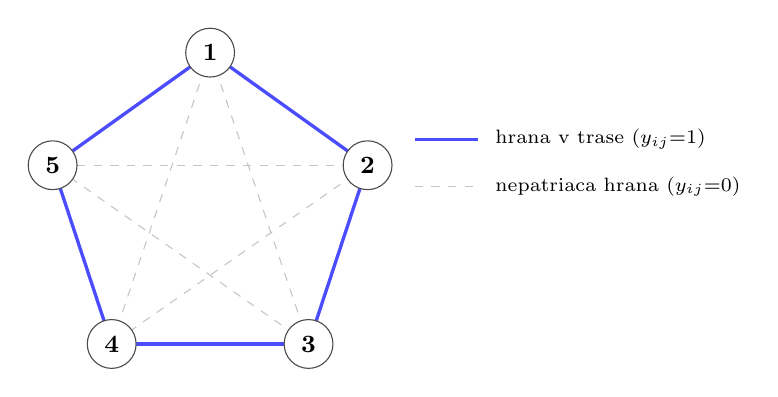
\begin{tikzpicture}[
    font=\small,
    vtx/.style={
        circle, draw=black!70, fill=white,
        minimum size=0.62cm, inner sep=1pt,
        font=\small\bfseries
    },
    touredge/.style={draw=blue!70, very thick},
    nonedge/.style={draw=gray!45, dashed, thin}
]

%% Vrcholy pravidelného päťuholníka r=2.1, stred=(2.60, 2.50)
\coordinate (v1) at (2.60, 4.60);
\coordinate (v2) at (4.60, 3.17);
\coordinate (v3) at (3.85, 0.90);
\coordinate (v4) at (1.35, 0.90);
\coordinate (v5) at (0.60, 3.17);

%% ── Diagonály (non-tour, y=0) ────────────────────────────────────
\draw[nonedge] (v1) -- (v3);
\draw[nonedge] (v1) -- (v4);
\draw[nonedge] (v2) -- (v4);
\draw[nonedge] (v2) -- (v5);
\draw[nonedge] (v3) -- (v5);

%% ── Vonkajší päťuholník (tour, y=1) ─────────────────────────────
\draw[touredge] (v1) -- (v2);
\draw[touredge] (v2) -- (v3);
\draw[touredge] (v3) -- (v4);
\draw[touredge] (v4) -- (v5);
\draw[touredge] (v5) -- (v1);

%% ── Vrcholy ──────────────────────────────────────────────────────
\node[vtx] at (v1) {1};
\node[vtx] at (v2) {2};
\node[vtx] at (v3) {3};
\node[vtx] at (v4) {4};
\node[vtx] at (v5) {5};

%% ── Legenda ──────────────────────────────────────────────────────
\draw[touredge] (5.20, 3.50) -- (6.00, 3.50);
\node[font=\scriptsize, anchor=west] at (6.10, 3.50)
    {hrana v trase (\(y_{ij}{=}1\))};
\draw[nonedge]  (5.20, 2.90) -- (6.00, 2.90);
\node[font=\scriptsize, anchor=west] at (6.10, 2.90)
    {nepatriaca hrana (\(y_{ij}{=}0\))};

\end{tikzpicture}}
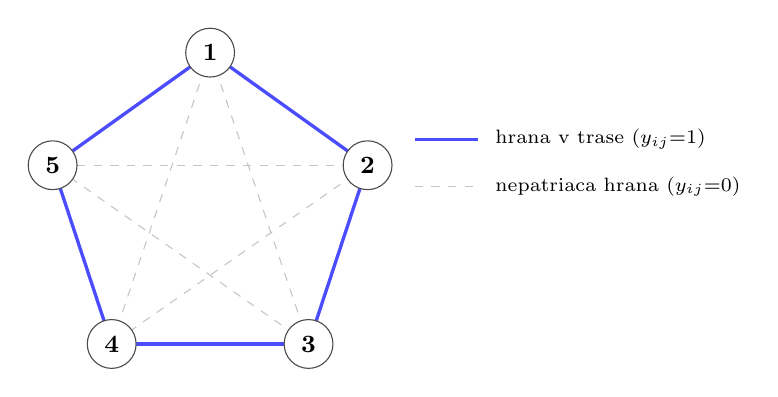
\begin{tikzpicture}[
    font=\small,
    vtx/.style={
        circle, draw=black!70, fill=white,
        minimum size=0.62cm, inner sep=1pt,
        font=\small\bfseries
    },
    touredge/.style={draw=blue!70, very thick},
    nonedge/.style={draw=gray!45, dashed, thin}
]

%% Vrcholy pravidelného päťuholníka r=2.1, stred=(2.60, 2.50)
\coordinate (v1) at (2.60, 4.60);
\coordinate (v2) at (4.60, 3.17);
\coordinate (v3) at (3.85, 0.90);
\coordinate (v4) at (1.35, 0.90);
\coordinate (v5) at (0.60, 3.17);

%% ── Diagonály (non-tour, y=0) ────────────────────────────────────
\draw[nonedge] (v1) -- (v3);
\draw[nonedge] (v1) -- (v4);
\draw[nonedge] (v2) -- (v4);
\draw[nonedge] (v2) -- (v5);
\draw[nonedge] (v3) -- (v5);

%% ── Vonkajší päťuholník (tour, y=1) ─────────────────────────────
\draw[touredge] (v1) -- (v2);
\draw[touredge] (v2) -- (v3);
\draw[touredge] (v3) -- (v4);
\draw[touredge] (v4) -- (v5);
\draw[touredge] (v5) -- (v1);

%% ── Vrcholy ──────────────────────────────────────────────────────
\node[vtx] at (v1) {1};
\node[vtx] at (v2) {2};
\node[vtx] at (v3) {3};
\node[vtx] at (v4) {4};
\node[vtx] at (v5) {5};

%% ── Legenda ──────────────────────────────────────────────────────
\draw[touredge] (5.20, 3.50) -- (6.00, 3.50);
\node[font=\scriptsize, anchor=west] at (6.10, 3.50)
    {hrana v trase (\(y_{ij}{=}1\))};
\draw[nonedge]  (5.20, 2.90) -- (6.00, 2.90);
\node[font=\scriptsize, anchor=west] at (6.10, 2.90)
    {nepatriaca hrana (\(y_{ij}{=}0\))};

\end{tikzpicture}}
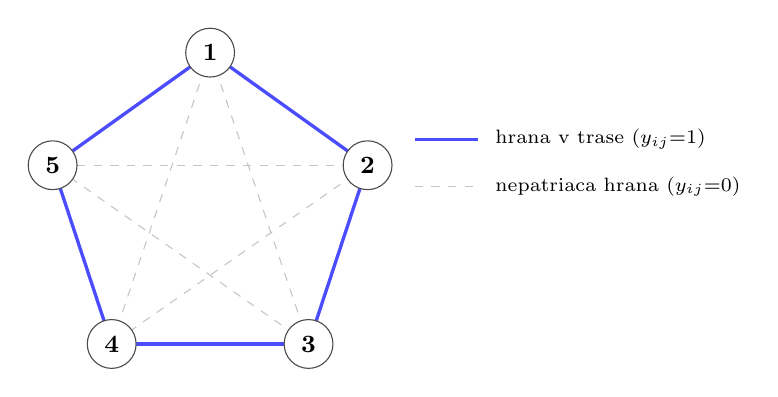
\begin{tikzpicture}[
    font=\small,
    vtx/.style={
        circle, draw=black!70, fill=white,
        minimum size=0.62cm, inner sep=1pt,
        font=\small\bfseries
    },
    touredge/.style={draw=blue!70, very thick},
    nonedge/.style={draw=gray!45, dashed, thin}
]

%% Vrcholy pravidelného päťuholníka r=2.1, stred=(2.60, 2.50)
\coordinate (v1) at (2.60, 4.60);
\coordinate (v2) at (4.60, 3.17);
\coordinate (v3) at (3.85, 0.90);
\coordinate (v4) at (1.35, 0.90);
\coordinate (v5) at (0.60, 3.17);

%% ── Diagonály (non-tour, y=0) ────────────────────────────────────
\draw[nonedge] (v1) -- (v3);
\draw[nonedge] (v1) -- (v4);
\draw[nonedge] (v2) -- (v4);
\draw[nonedge] (v2) -- (v5);
\draw[nonedge] (v3) -- (v5);

%% ── Vonkajší päťuholník (tour, y=1) ─────────────────────────────
\draw[touredge] (v1) -- (v2);
\draw[touredge] (v2) -- (v3);
\draw[touredge] (v3) -- (v4);
\draw[touredge] (v4) -- (v5);
\draw[touredge] (v5) -- (v1);

%% ── Vrcholy ──────────────────────────────────────────────────────
\node[vtx] at (v1) {1};
\node[vtx] at (v2) {2};
\node[vtx] at (v3) {3};
\node[vtx] at (v4) {4};
\node[vtx] at (v5) {5};

%% ── Legenda ──────────────────────────────────────────────────────
\draw[touredge] (5.20, 3.50) -- (6.00, 3.50);
\node[font=\scriptsize, anchor=west] at (6.10, 3.50)
    {hrana v trase (\(y_{ij}{=}1\))};
\draw[nonedge]  (5.20, 2.90) -- (6.00, 2.90);
\node[font=\scriptsize, anchor=west] at (6.10, 2.90)
    {nepatriaca hrana (\(y_{ij}{=}0\))};

\end{tikzpicture}}
    \caption{Odvodenie binárnych štítkov z referenčnej trasy na príklade
             úplného grafu \(K_5\): hrany turu sú označené \(y_{ij}=1\),
             ostatné \(y_{ij}=0\).}
    \label{fig:edge_label_derivation}
\end{figure}

\indent Keďže Hamiltonovský cyklus obsahuje presne \(n\) hrán a úplný
graf ich má \(m = n(n-1)/2\), pozitívnych štítkov je výrazne menej ako
negatívnych. Tento nepomer priamo motivuje použitie váženej straty pri
trénovaní modelov, opísanej v sekcii~\ref{sec:trenovanie}.

%% ═══════════════════════════════════════════════════════════════════════════
%% 3.5  MODELOVÉ ARCHITEKTÚRY
%% ═══════════════════════════════════════════════════════════════════════════
\section{Modelové architektúry}
\label{sec:modelove_architektury}

\indent V tejto práci boli navrhnuté a porovnané tri rodiny neurónových
modelov. Všetky plnia rovnakú úlohu: na základe vektora geometrických
príznakov hrany \(\phi_{ij}\) odhadnúť skóre \(s_{ij}\), ktoré vyjadruje,
nakoľko pravdepodobne daná hrana patrí do výslednej trasy. Rodiny sa líšia
tým, \emph{koľko kontextu} o celej inštancii môže každý model pri tomto
odhade využiť.

\indent Neurónové siete sú trieda modelov strojového učenia inšpirovaná
spôsobom, akým biologické neuróny spracovávajú a prenášajú signály.
Základnou stavebnou jednotkou je \emph{umelý neurón} — funkcia, ktorá
prijíma niekoľko vstupných hodnôt, vypočíta ich váženú sumu a výsledok
transformuje nelineárnou \emph{aktivačnou funkciou}. Tá je kľúčová:
bez nej by sieť akejkoľvek hĺbky zostávala ekvivalentná jednej lineárnej
transformácii a nebola by schopná zachytiť zložité vzory v dátach.
V tejto práci sa používajú dve aktivačné funkcie: \textbf{ReLU},
ktorá záporné hodnoty nahradí nulou, a \textbf{GELU}, jej hladká
aproximácia s lepšími vlastnosťami pri trénovaní hlbokých sietí.

\indent Neuróny sa usporadúvajú do \emph{vrstiev}. Každá vrstva prijíma
výstupy predchádzajúcej vrstvy, transformuje ich a odovzdáva ďalej. Sieť
zložená z viacerých vrstiev za sebou sa nazýva \emph{viacvrstvový
perceptrón} (MLP). Čím viac vrstiev, tým abstraktnejšie vzory môže model
zachytiť — nižšie vrstvy sa učia jednoduché lokálne vlastnosti, vyššie
ich kombinujú do zložitejších konceptov.

\indent Váhy siete sa nastavujú počas \emph{trénovania}: model opakuje
predikcie nad trénovacími príkladmi, meria odchýlku od správnych hodnôt
pomocou \emph{stratovej funkcie} a algoritmom \emph{spätného šírenia}
posúva váhy smerom, ktorý chybu znižuje.
\textbf{Vrstvová normalizácia} (LayerNorm) priebežne upravuje rozsah
aktivácií v hlbokých sieťach a \textbf{Dropout} počas trénovania
náhodne deaktivuje časť neurónov, čím znižuje riziko preučenia.

\indent V kontexte tejto práce prijíma každý model vektor príznakov
hrany \(\phi_{ij}\) a vydáva jedno číslo — skóre \(s_{ij}\). Tri
porovnávané rodiny sa líšia predovšetkým tým, či pri hodnotení hrany
uvažujú len o nej samotnej, alebo zohľadňujú aj informáciu z celej
inštancie. Tabuľka~\ref{tab:arch_porovnanie} sumarizuje kľúčové
vlastnosti každej z nich.

\begin{table}[H]
\centering
\caption{Porovnanie troch porovnávaných architektúr neurónových modelov.}
\label{tab:arch_porovnanie}
\begin{tabular}{lp{2.6cm}p{2.6cm}p{3.2cm}}
\hline
\textbf{Vlastnosť}       & \textbf{EdgeMLP}               & \textbf{EdgeResMLP}            & \textbf{EdgeTransformer}         \\ \hline
Vstup                    & \(\phi_{ij}\in\mathbb{R}^{10}\) & \(\phi_{ij}\in\mathbb{R}^{10}\) & \(\phi_{ij}\in\mathbb{R}^{10}\)  \\
Spracovanie hrany        & lokálne, nezávislé             & lokálne, nezávislé             & globálne + lokálne               \\
Kontext inštancie        & žiadny                         & žiadny                         & celá inštancia                   \\
Aktivácia                & ReLU                           & GELU                           & GELU                             \\
Reziduálne spojenia      & nie                            & áno                            & áno (attn + FFN)                 \\
Hĺbka (vrstvy / bloky)  & 2 alebo 3                      & 4                              & 3                                \\
Skryté dimenzie          & 128 alebo 256                  & 128                            & 128                              \\
Hlavy pozornosti         & —                              & —                              & 4                                \\ \hline
\end{tabular}
\end{table}

%% ─── 3.5.1  Viacvrstvový perceptrón nad hranami ──────────────────────────
\subsection{Viacvrstvový perceptrón nad hranami}
\label{sec:edge_mlp}

\indent Najjednoduchšiu rodinu tvoril hranový MLP, v ktorom sa každá
hrana spracovávala úplne nezávisle od všetkých ostatných. Vektor
príznakov hrany \(\phi_{ij}\) postupne prešiel niekoľkými vrstvami
lineárnych transformácií s aktiváciou ReLU. Každá vrstva kombinuje
vstupné hodnoty, aplikuje nelinearitu a odovzdáva výsledok ďalšej.
Po poslednej skrytej vrstve záverečná lineárna projekcia vyprodukovala
skalárne skóre hrany \(s_{ij}\).

\begin{figure}[H]
    \centering
    \resizebox{0.72\textwidth}{!}{% mlp_edge_diagram.tex
% Schéma hranového MLP modelu (EdgeMLP)
% Použitie: \resizebox{0.72\textwidth}{!}{% mlp_edge_diagram.tex
% Schéma hranového MLP modelu (EdgeMLP)
% Použitie: \resizebox{0.72\textwidth}{!}{% mlp_edge_diagram.tex
% Schéma hranového MLP modelu (EdgeMLP)
% Použitie: \resizebox{0.72\textwidth}{!}{\input{figures/tikz/mlp_edge_diagram}}
\begin{tikzpicture}[
    font=\small,
    box/.style={
        draw, rounded corners=5pt, align=center,
        minimum width=3.4cm, minimum height=0.82cm,
        inner sep=4pt
    },
    inputbox/.style={box, fill=gray!10, draw=gray!50},
    layerbox/.style={box, fill=blue!8, draw=blue!40},
    outbox/.style={box, fill=green!8, draw=green!50},
    labelbox/.style={font=\scriptsize\itshape, text=gray!60, align=left,
                     text width=4.0cm},
    arrow/.style={-{Latex[length=2.5mm]}, thick}
]

\node[inputbox] (phi) at (0, 0)
    {\(\phi_{ij} \in \mathbb{R}^{10}\)\\[-2pt]
     \scriptsize vektor príznakov hrany};

\node[layerbox] (h1) at (0, -1.55)
    {Lineárna vrstva\\[-2pt]
     \scriptsize + aktivácia ReLU};

\node[layerbox] (hdots) at (0, -3.10)
    {\(\cdots\)\\[-2pt]
     \scriptsize (opakuje sa \(D\)-krát)};

\node[layerbox] (hD) at (0, -4.65)
    {Lineárna vrstva\\[-2pt]
     \scriptsize + aktivácia ReLU};

\node[outbox] (out) at (0, -6.15)
    {Záverečná projekcia\\[-2pt]
     \scriptsize logit \(s_{ij} \in \mathbb{R}\)};

\draw[arrow] (phi)   -- (h1);
\draw[arrow] (h1)    -- (hdots);
\draw[arrow] (hdots) -- (hD);
\draw[arrow] (hD)    -- (out);

\node[labelbox, anchor=north west] at (2.5, -0.25)
    {\textbf{Vstup:} 10-rozmerný vektor
     obsahujúci polohu oboch vrcholov,
     vzdialenosť, relatívnu geometriu
     a uhol hrany.};

\node[labelbox, anchor=north west] at (2.5, -2.00)
    {\textbf{Skryté vrstvy:} každá vrstva
     lineárne transformuje vstup
     a aplikuje ReLU nelinearitu.};

\node[labelbox, anchor=north west] at (2.5, -5.25)
    {\textbf{Výstup:} jediné číslo
     (logit) vyjadrujúce
     odhadovanú príslušnosť
     hrany k optimálnej trase.};

\node[draw=gray!35, rounded corners=4pt, fill=gray!5,
      font=\scriptsize, align=center, text width=6.5cm,
      inner sep=5pt] at (0, -7.55)
    {Každá hrana \(\{i,j\}\) sa spracováva \textbf{nezávisle} —
     model pri hodnotení hrany nemá prístup k informácii
     o ostatných hranách ani vrcholoch inštancie.};

\end{tikzpicture}
}
\begin{tikzpicture}[
    font=\small,
    box/.style={
        draw, rounded corners=5pt, align=center,
        minimum width=3.4cm, minimum height=0.82cm,
        inner sep=4pt
    },
    inputbox/.style={box, fill=gray!10, draw=gray!50},
    layerbox/.style={box, fill=blue!8, draw=blue!40},
    outbox/.style={box, fill=green!8, draw=green!50},
    labelbox/.style={font=\scriptsize\itshape, text=gray!60, align=left,
                     text width=4.0cm},
    arrow/.style={-{Latex[length=2.5mm]}, thick}
]

\node[inputbox] (phi) at (0, 0)
    {\(\phi_{ij} \in \mathbb{R}^{10}\)\\[-2pt]
     \scriptsize vektor príznakov hrany};

\node[layerbox] (h1) at (0, -1.55)
    {Lineárna vrstva\\[-2pt]
     \scriptsize + aktivácia ReLU};

\node[layerbox] (hdots) at (0, -3.10)
    {\(\cdots\)\\[-2pt]
     \scriptsize (opakuje sa \(D\)-krát)};

\node[layerbox] (hD) at (0, -4.65)
    {Lineárna vrstva\\[-2pt]
     \scriptsize + aktivácia ReLU};

\node[outbox] (out) at (0, -6.15)
    {Záverečná projekcia\\[-2pt]
     \scriptsize logit \(s_{ij} \in \mathbb{R}\)};

\draw[arrow] (phi)   -- (h1);
\draw[arrow] (h1)    -- (hdots);
\draw[arrow] (hdots) -- (hD);
\draw[arrow] (hD)    -- (out);

\node[labelbox, anchor=north west] at (2.5, -0.25)
    {\textbf{Vstup:} 10-rozmerný vektor
     obsahujúci polohu oboch vrcholov,
     vzdialenosť, relatívnu geometriu
     a uhol hrany.};

\node[labelbox, anchor=north west] at (2.5, -2.00)
    {\textbf{Skryté vrstvy:} každá vrstva
     lineárne transformuje vstup
     a aplikuje ReLU nelinearitu.};

\node[labelbox, anchor=north west] at (2.5, -5.25)
    {\textbf{Výstup:} jediné číslo
     (logit) vyjadrujúce
     odhadovanú príslušnosť
     hrany k optimálnej trase.};

\node[draw=gray!35, rounded corners=4pt, fill=gray!5,
      font=\scriptsize, align=center, text width=6.5cm,
      inner sep=5pt] at (0, -7.55)
    {Každá hrana \(\{i,j\}\) sa spracováva \textbf{nezávisle} —
     model pri hodnotení hrany nemá prístup k informácii
     o ostatných hranách ani vrcholoch inštancie.};

\end{tikzpicture}
}
\begin{tikzpicture}[
    font=\small,
    box/.style={
        draw, rounded corners=5pt, align=center,
        minimum width=3.4cm, minimum height=0.82cm,
        inner sep=4pt
    },
    inputbox/.style={box, fill=gray!10, draw=gray!50},
    layerbox/.style={box, fill=blue!8, draw=blue!40},
    outbox/.style={box, fill=green!8, draw=green!50},
    labelbox/.style={font=\scriptsize\itshape, text=gray!60, align=left,
                     text width=4.0cm},
    arrow/.style={-{Latex[length=2.5mm]}, thick}
]

\node[inputbox] (phi) at (0, 0)
    {\(\phi_{ij} \in \mathbb{R}^{10}\)\\[-2pt]
     \scriptsize vektor príznakov hrany};

\node[layerbox] (h1) at (0, -1.55)
    {Lineárna vrstva\\[-2pt]
     \scriptsize + aktivácia ReLU};

\node[layerbox] (hdots) at (0, -3.10)
    {\(\cdots\)\\[-2pt]
     \scriptsize (opakuje sa \(D\)-krát)};

\node[layerbox] (hD) at (0, -4.65)
    {Lineárna vrstva\\[-2pt]
     \scriptsize + aktivácia ReLU};

\node[outbox] (out) at (0, -6.15)
    {Záverečná projekcia\\[-2pt]
     \scriptsize logit \(s_{ij} \in \mathbb{R}\)};

\draw[arrow] (phi)   -- (h1);
\draw[arrow] (h1)    -- (hdots);
\draw[arrow] (hdots) -- (hD);
\draw[arrow] (hD)    -- (out);

\node[labelbox, anchor=north west] at (2.5, -0.25)
    {\textbf{Vstup:} 10-rozmerný vektor
     obsahujúci polohu oboch vrcholov,
     vzdialenosť, relatívnu geometriu
     a uhol hrany.};

\node[labelbox, anchor=north west] at (2.5, -2.00)
    {\textbf{Skryté vrstvy:} každá vrstva
     lineárne transformuje vstup
     a aplikuje ReLU nelinearitu.};

\node[labelbox, anchor=north west] at (2.5, -5.25)
    {\textbf{Výstup:} jediné číslo
     (logit) vyjadrujúce
     odhadovanú príslušnosť
     hrany k optimálnej trase.};

\node[draw=gray!35, rounded corners=4pt, fill=gray!5,
      font=\scriptsize, align=center, text width=6.5cm,
      inner sep=5pt] at (0, -7.55)
    {Každá hrana \(\{i,j\}\) sa spracováva \textbf{nezávisle} —
     model pri hodnotení hrany nemá prístup k informácii
     o ostatných hranách ani vrcholoch inštancie.};

\end{tikzpicture}
}
    \caption{Schéma hranového MLP modelu. Vektor príznakov hrany
             \(\phi_{ij}\) prechádza sekvenciou lineárnych vrstiev
             s aktiváciou ReLU. Každá hrana sa spracováva nezávisle
             — model nemá informáciu o zvyšku grafu.}
    \label{fig:mlp_edge_diagram}
\end{figure}

\indent Výhodou tohto prístupu bola výpočtová jednoduchosť: celú
inštanciu bolo možné spracovať ako jednu dávku vektorov naraz, bez
akéhokoľvek sekvenčného algoritmu. Nevýhodou bolo, že model pri
hodnotení každej hrany nemal prístup k žiadnej informácii o zvyšku
grafu. V experimentoch sa testovali dve varianty tejto rodiny —
plytší model s dvoma skrytými vrstvami (\texttt{edge\_mlp},
\(d_h = 128\)) a hlbší model s tromi vrstvami a väčšou kapacitou
(\texttt{edge\_mlp\_deep}, \(d_h = 256\)).

%% ─── 3.5.2  Reziduálny MLP model ─────────────────────────────────────────
\subsection{Reziduálny MLP model}
\label{sec:edge_res_mlp}

\indent Druhú rodinu tvoril reziduálny MLP, ktorý rozšíril základný
prístup o dve dôležité vylepšenia. Namiesto jednoduchej sekvencie vrstiev
sieť pracovala s \emph{reziduálnymi blokmi}: každý blok sa neučil celé
zobrazenie vstupu na výstup, ale iba \emph{korekciu} voči tomu, čo
sa na vstup bloku priviedlo. Výstup bloku bol teda súčtom jeho vstupu
a naučenej korekcie — odtiaľ názov reziduálna (zvyšková) sieť
\parencite{he2016resnet}. Vnútri každého bloku sa navyše uplatnila
vrstvová normalizácia pred transformáciou a náhodné vypúšťanie za ňou.

\begin{figure}[H]
    \centering
    \resizebox{0.80\textwidth}{!}{% res_mlp_diagram.tex
% Diagram reziduálneho MLP modelu s vysvetlením LayerNorm a Dropout
% Použitie: \resizebox{0.80\textwidth}{!}{% res_mlp_diagram.tex
% Diagram reziduálneho MLP modelu s vysvetlením LayerNorm a Dropout
% Použitie: \resizebox{0.80\textwidth}{!}{% res_mlp_diagram.tex
% Diagram reziduálneho MLP modelu s vysvetlením LayerNorm a Dropout
% Použitie: \resizebox{0.80\textwidth}{!}{\input{figures/tikz/res_mlp_diagram}}
\begin{tikzpicture}[
    font=\small,
    box/.style={
        draw, rounded corners=5pt, align=center,
        minimum width=3.4cm, minimum height=0.82cm,
        inner sep=4pt
    },
    inputbox/.style={box, fill=gray!10, draw=gray!50},
    projbox/.style={box, fill=blue!8, draw=blue!40},
    normbox/.style={box, fill=yellow!10, draw=yellow!60!black},
    dropbox/.style={box, fill=red!6, draw=red!30},
    outbox/.style={box, fill=green!8, draw=green!50},
    labelbox/.style={font=\scriptsize\itshape, text=gray!65, align=left,
                     text width=4.2cm},
    arrow/.style={-{Latex[length=2.5mm]}, thick},
    resarrow/.style={-{Latex[length=2.5mm]}, thick, draw=green!55!black}
]

\node[inputbox] (phi) at (0, 0)
    {\(\phi_{ij} \in \mathbb{R}^{10}\)\\[-2pt]
     \scriptsize vektor príznakov hrany};

\node[projbox] (proj) at (0, -1.55)
    {Vstupná projekcia\\[-2pt]
     \scriptsize + aktivácia GELU};

\node[normbox] (ln1) at (0, -3.10)
    {Vrstvová normalizácia\\[-2pt]
     \scriptsize (LayerNorm)};

\node[projbox] (fc1) at (0, -4.50)
    {Lineárna transformácia\\[-2pt]
     \scriptsize + aktivácia GELU};

\node[dropbox] (drop) at (0, -5.85)
    {Náhodné vypúšťanie\\[-2pt]
     \scriptsize (Dropout)};

\node[projbox] (fc2) at (0, -7.20)
    {Lineárna transformácia};

\node[draw=green!55!black, fill=green!5, circle,
      minimum size=0.65cm, font=\bfseries\small] (plus) at (0, -8.55) {+};

\draw[draw=green!40, dashed, rounded corners=6pt]
    (-2.3, -2.55) rectangle (2.3, -7.85);
\node[font=\scriptsize\itshape, text=green!60!black]
    at (0, -2.38) {reziduálny blok (opakuje sa \(D\)-krát)};

\draw[resarrow]
    (proj.east) -- ++(1.4, 0) -- ++(0, -7.0) -- (plus.east);
\node[font=\scriptsize, text=green!60!black, rotate=90, anchor=south]
    at (3.0, -5.2) {reziduálna skratka};

\node[outbox] (out) at (0, -9.95)
    {Záverečná lineárna vrstva\\[-2pt]
     \scriptsize logit \(s_{ij} \in \mathbb{R}\)};

\draw[arrow] (phi)  -- (proj);
\draw[arrow] (proj) -- (ln1);
\draw[arrow] (ln1)  -- (fc1);
\draw[arrow] (fc1)  -- (drop);
\draw[arrow] (drop) -- (fc2);
\draw[arrow] (fc2)  -- (plus);
\draw[arrow] (plus) -- (out);

\node[labelbox, anchor=north west] at (3.5, -3.25)
    {\textbf{LayerNorm:} normalizuje aktivácie
     v rámci jedného vzorku — stabilizuje tréning
     a urýchľuje konvergenciu.};

\node[labelbox, anchor=north west] at (3.5, -5.85)
    {\textbf{Dropout:} náhodne deaktivuje
     časť neurónov — zabraňuje preučeniu.};

\node[labelbox, anchor=north west] at (3.5, -8.55)
    {\textbf{Reziduálna skratka:}
     gradient prúdi priamo, bez
     útlmu cez hlboké bloky.};

\end{tikzpicture}
}
\begin{tikzpicture}[
    font=\small,
    box/.style={
        draw, rounded corners=5pt, align=center,
        minimum width=3.4cm, minimum height=0.82cm,
        inner sep=4pt
    },
    inputbox/.style={box, fill=gray!10, draw=gray!50},
    projbox/.style={box, fill=blue!8, draw=blue!40},
    normbox/.style={box, fill=yellow!10, draw=yellow!60!black},
    dropbox/.style={box, fill=red!6, draw=red!30},
    outbox/.style={box, fill=green!8, draw=green!50},
    labelbox/.style={font=\scriptsize\itshape, text=gray!65, align=left,
                     text width=4.2cm},
    arrow/.style={-{Latex[length=2.5mm]}, thick},
    resarrow/.style={-{Latex[length=2.5mm]}, thick, draw=green!55!black}
]

\node[inputbox] (phi) at (0, 0)
    {\(\phi_{ij} \in \mathbb{R}^{10}\)\\[-2pt]
     \scriptsize vektor príznakov hrany};

\node[projbox] (proj) at (0, -1.55)
    {Vstupná projekcia\\[-2pt]
     \scriptsize + aktivácia GELU};

\node[normbox] (ln1) at (0, -3.10)
    {Vrstvová normalizácia\\[-2pt]
     \scriptsize (LayerNorm)};

\node[projbox] (fc1) at (0, -4.50)
    {Lineárna transformácia\\[-2pt]
     \scriptsize + aktivácia GELU};

\node[dropbox] (drop) at (0, -5.85)
    {Náhodné vypúšťanie\\[-2pt]
     \scriptsize (Dropout)};

\node[projbox] (fc2) at (0, -7.20)
    {Lineárna transformácia};

\node[draw=green!55!black, fill=green!5, circle,
      minimum size=0.65cm, font=\bfseries\small] (plus) at (0, -8.55) {+};

\draw[draw=green!40, dashed, rounded corners=6pt]
    (-2.3, -2.55) rectangle (2.3, -7.85);
\node[font=\scriptsize\itshape, text=green!60!black]
    at (0, -2.38) {reziduálny blok (opakuje sa \(D\)-krát)};

\draw[resarrow]
    (proj.east) -- ++(1.4, 0) -- ++(0, -7.0) -- (plus.east);
\node[font=\scriptsize, text=green!60!black, rotate=90, anchor=south]
    at (3.0, -5.2) {reziduálna skratka};

\node[outbox] (out) at (0, -9.95)
    {Záverečná lineárna vrstva\\[-2pt]
     \scriptsize logit \(s_{ij} \in \mathbb{R}\)};

\draw[arrow] (phi)  -- (proj);
\draw[arrow] (proj) -- (ln1);
\draw[arrow] (ln1)  -- (fc1);
\draw[arrow] (fc1)  -- (drop);
\draw[arrow] (drop) -- (fc2);
\draw[arrow] (fc2)  -- (plus);
\draw[arrow] (plus) -- (out);

\node[labelbox, anchor=north west] at (3.5, -3.25)
    {\textbf{LayerNorm:} normalizuje aktivácie
     v rámci jedného vzorku — stabilizuje tréning
     a urýchľuje konvergenciu.};

\node[labelbox, anchor=north west] at (3.5, -5.85)
    {\textbf{Dropout:} náhodne deaktivuje
     časť neurónov — zabraňuje preučeniu.};

\node[labelbox, anchor=north west] at (3.5, -8.55)
    {\textbf{Reziduálna skratka:}
     gradient prúdi priamo, bez
     útlmu cez hlboké bloky.};

\end{tikzpicture}
}
\begin{tikzpicture}[
    font=\small,
    box/.style={
        draw, rounded corners=5pt, align=center,
        minimum width=3.4cm, minimum height=0.82cm,
        inner sep=4pt
    },
    inputbox/.style={box, fill=gray!10, draw=gray!50},
    projbox/.style={box, fill=blue!8, draw=blue!40},
    normbox/.style={box, fill=yellow!10, draw=yellow!60!black},
    dropbox/.style={box, fill=red!6, draw=red!30},
    outbox/.style={box, fill=green!8, draw=green!50},
    labelbox/.style={font=\scriptsize\itshape, text=gray!65, align=left,
                     text width=4.2cm},
    arrow/.style={-{Latex[length=2.5mm]}, thick},
    resarrow/.style={-{Latex[length=2.5mm]}, thick, draw=green!55!black}
]

\node[inputbox] (phi) at (0, 0)
    {\(\phi_{ij} \in \mathbb{R}^{10}\)\\[-2pt]
     \scriptsize vektor príznakov hrany};

\node[projbox] (proj) at (0, -1.55)
    {Vstupná projekcia\\[-2pt]
     \scriptsize + aktivácia GELU};

\node[normbox] (ln1) at (0, -3.10)
    {Vrstvová normalizácia\\[-2pt]
     \scriptsize (LayerNorm)};

\node[projbox] (fc1) at (0, -4.50)
    {Lineárna transformácia\\[-2pt]
     \scriptsize + aktivácia GELU};

\node[dropbox] (drop) at (0, -5.85)
    {Náhodné vypúšťanie\\[-2pt]
     \scriptsize (Dropout)};

\node[projbox] (fc2) at (0, -7.20)
    {Lineárna transformácia};

\node[draw=green!55!black, fill=green!5, circle,
      minimum size=0.65cm, font=\bfseries\small] (plus) at (0, -8.55) {+};

\draw[draw=green!40, dashed, rounded corners=6pt]
    (-2.3, -2.55) rectangle (2.3, -7.85);
\node[font=\scriptsize\itshape, text=green!60!black]
    at (0, -2.38) {reziduálny blok (opakuje sa \(D\)-krát)};

\draw[resarrow]
    (proj.east) -- ++(1.4, 0) -- ++(0, -7.0) -- (plus.east);
\node[font=\scriptsize, text=green!60!black, rotate=90, anchor=south]
    at (3.0, -5.2) {reziduálna skratka};

\node[outbox] (out) at (0, -9.95)
    {Záverečná lineárna vrstva\\[-2pt]
     \scriptsize logit \(s_{ij} \in \mathbb{R}\)};

\draw[arrow] (phi)  -- (proj);
\draw[arrow] (proj) -- (ln1);
\draw[arrow] (ln1)  -- (fc1);
\draw[arrow] (fc1)  -- (drop);
\draw[arrow] (drop) -- (fc2);
\draw[arrow] (fc2)  -- (plus);
\draw[arrow] (plus) -- (out);

\node[labelbox, anchor=north west] at (3.5, -3.25)
    {\textbf{LayerNorm:} normalizuje aktivácie
     v rámci jedného vzorku — stabilizuje tréning
     a urýchľuje konvergenciu.};

\node[labelbox, anchor=north west] at (3.5, -5.85)
    {\textbf{Dropout:} náhodne deaktivuje
     časť neurónov — zabraňuje preučeniu.};

\node[labelbox, anchor=north west] at (3.5, -8.55)
    {\textbf{Reziduálna skratka:}
     gradient prúdi priamo, bez
     útlmu cez hlboké bloky.};

\end{tikzpicture}
}
    \caption{Schéma reziduálneho MLP modelu. Vstup prechádza vstupnou
             projekciou a následne sekvenciou reziduálnych blokov.
             Každý blok aplikuje vrstvovú normalizáciu, dve lineárne
             transformácie s aktiváciou GELU a náhodné vypúšťanie.
             Reziduálna skratka sčíta vstup bloku s jeho výstupom.}
    \label{fig:res_mlp_diagram}
\end{figure}

\indent Reziduálne zapojenie prináša dva praktické prínosy. Po prvé,
gradient môže prúdiť reziduálnymi skratkami priamo naprieč celou
hĺbkou siete bez toho, aby sa rozptýlil alebo explodoval — to umožňuje
stabilné trénovanie aj pri väčšom počte blokov. Po druhé, vrstvová
normalizácia udržiava aktivácie v zdravom rozsahu. Rovnako ako základný
MLP, aj tento model zostával \emph{lokálnym}: každá hrana sa
spracovávala nezávisle a model nemal priamy prístup ku kontextu zvyšku
grafu. Model bol konfigurovaný so štyrmi reziduálnymi blokmi
a skrytou dimenziou \(d_h = 128\).

%% ─── 3.5.3  Transformerový model s hranovým výstupom ────────────────────
\subsection{Transformerový model s hranovým výstupom}
\label{sec:edge_transformer}

\indent Tretiu a najzložitejšiu rodinu tvoril kontextový transformerový
model, ktorý ako jediný pracoval s \emph{globálnym kontextom} celej
inštancie. Namiesto toho, aby hodnotil každú hranu izolovane, model
najprv zostavil reprezentácie všetkých vrcholov s ohľadom na ich
vzájomné vzťahy — a až potom ohodnotil každú hranu.

\indent Model pracoval v dvoch fázach. V prvej fáze sa zo súradníc
každého mesta zostavila jeho vnútorná reprezentácia, ktorá sa následne
opakovane aktualizovala \emph{mechanizmom vlastnej pozornosti}
(self-attention). Tento mechanizmus umožňuje každému vrcholu
„zobrať do úvahy" všetky ostatné vrcholy inštancie a podľa toho
upraviť svoju vlastnú reprezentáciu, inšpirujúc sa transformerovou
architektúrou \parencite{vaswani2017attention}.
Výsledkom je, že každý vrchol nesie \emph{kontextovú reprezentáciu}
zakódovávajúcu nielen jeho vlastnú polohu, ale aj jeho vzťah
ku všetkým ostatným mestám. V druhej fáze sa pre každú hranu zlúčili
kontextové reprezentácie oboch jej krajných vrcholov spolu
s pôvodnými geometrickými príznakmi hrany. Toto zlúčenie vstúpilo
do výstupnej siete, ktorá vyprodukovala skóre hrany \(s_{ij}\).

\begin{figure}[H]
    \centering
    \resizebox{0.95\textwidth}{!}{% transformer_diagram.tex
% Diagram transformerového modelu — dve fázy, konceptuálny
% Použitie: \resizebox{0.88\textwidth}{!}{% transformer_diagram.tex
% Diagram transformerového modelu — dve fázy, konceptuálny
% Použitie: \resizebox{0.88\textwidth}{!}{% transformer_diagram.tex
% Diagram transformerového modelu — dve fázy, konceptuálny
% Použitie: \resizebox{0.88\textwidth}{!}{\input{figures/tikz/transformer_diagram}}
\begin{tikzpicture}[
    font=\small,
    box/.style={
        draw, rounded corners=5pt, align=center,
        minimum width=3.6cm, minimum height=0.85cm,
        inner sep=5pt
    },
    inputbox/.style={box, fill=gray!10, draw=gray!50},
    attnbox/.style={box, fill=orange!10, draw=orange!50},
    mergebox/.style={box, fill=purple!8, draw=purple!40},
    outbox/.style={box, fill=green!8, draw=green!50},
    labelbox/.style={font=\scriptsize\itshape, text=gray!65, align=left,
                     text width=5.0cm},
    arrow/.style={-{Latex[length=2.5mm]}, thick},
    dasharrow/.style={-{Latex[length=2mm]}, dashed, gray!60}
]

%% ══════════════════════════════════════════════════════════════════
%% FÁZA 1 — Kódovanie vrcholov
%% ══════════════════════════════════════════════════════════════════
\node[font=\bfseries\small, text=orange!70!black]
    at (0, 0.55) {Fáza 1 — kódovanie vrcholov};

\node[inputbox] (coords) at (0, -0.45)
    {Súradnice miest \((u_i, v_i)\)\\[-2pt]
     \scriptsize pre všetky vrcholy inštancie};

\node[attnbox] (embed) at (0, -2.00)
    {Lineárna projekcia\\[-2pt]
     \scriptsize súradnice → vnútorná reprezentácia};

\node[attnbox] (attn) at (0, -3.55)
    {Mechanizmus vlastnej pozornosti\\[-2pt]
     \scriptsize každý vrchol "sleduje" všetky ostatné};

\node[attnbox] (repeat) at (0, -5.10)
    {\(\cdots\) opakuje sa \(L\)-krát};

\node[outbox] (ctx) at (0, -6.55)
    {Kontextové reprezentácie \(z_i\)\\[-2pt]
     \scriptsize vrchol = poloha + vzťah k ostatným};

\draw[arrow] (coords) -- (embed);
\draw[arrow] (embed)  -- (attn);
\draw[arrow] (attn)   -- (repeat);
\draw[arrow] (repeat) -- (ctx);

%% Ohraničenie fázy 1
\draw[draw=orange!35, rounded corners=6pt, dashed]
    (-2.5, 0.20) rectangle (2.5, -7.20);

%% ══════════════════════════════════════════════════════════════════
%% FÁZA 2 — Skórovanie hrán
%% ══════════════════════════════════════════════════════════════════
\node[font=\bfseries\small, text=purple!70!black]
    at (7.0, 0.55) {Fáza 2 — skórovanie hrán};

%% Vstupné zdroje pre hranu {i,j}
\node[outbox] (zi) at (5.5, -0.45)
    {\(z_i\) — kontext vrcholu \(i\)};
\node[outbox] (zj) at (8.5, -0.45)
    {\(z_j\) — kontext vrcholu \(j\)};
\node[inputbox] (phi) at (7.0, -2.00)
    {\(\phi_{ij}\) — príznaky hrany};

%% Spojenie
\node[mergebox] (merge) at (7.0, -3.55)
    {Zlúčenie informácií\\[-2pt]
     \scriptsize kontext + príznaky hrany};

\node[mergebox] (head) at (7.0, -5.10)
    {Výstupná sieť\\[-2pt]
     \scriptsize (dve lineárne vrstvy + GELU)};

\node[outbox] (score) at (7.0, -6.55)
    {Skóre hrany \(s_{ij} \in \mathbb{R}\)\\[-2pt]
     \scriptsize miera príslušnosti k trase};

\draw[arrow] (zi)    |- (merge);
\draw[arrow] (zj)    |- (merge);
\draw[arrow] (phi)   -- (merge);
\draw[arrow] (merge) -- (head);
\draw[arrow] (head)  -- (score);

%% Prepojenie fázy 1 → fáza 2
\draw[arrow, draw=orange!60] (ctx.east) -- ++(1.0,0)
    |- node[midway, above, font=\scriptsize, text=orange!70]
       {pre každú hranu} (zi.west);
\draw[arrow, draw=orange!60] (ctx.east) -- ++(1.0,0)
    |- (zj.west);

%% Ohraničenie fázy 2
\draw[draw=purple!30, rounded corners=6pt, dashed]
    (4.2, 0.20) rectangle (9.8, -7.20);

%% ── Vysvetlivka dole ─────────────────────────────────────────────
\node[font=\scriptsize, text=gray!65, align=center, text width=13cm]
    at (3.5, -8.10)
    {Kľúčový rozdiel oproti MLP: transformer najprv zostaví
     \emph{globálny kontext} celej inštancie (Fáza 1) a až potom
     hodnotí každú hranu — s vedomosťou o jej vzťahu ku všetkým
     ostatným vrcholom (Fáza 2).};

\end{tikzpicture}}
\begin{tikzpicture}[
    font=\small,
    box/.style={
        draw, rounded corners=5pt, align=center,
        minimum width=3.6cm, minimum height=0.85cm,
        inner sep=5pt
    },
    inputbox/.style={box, fill=gray!10, draw=gray!50},
    attnbox/.style={box, fill=orange!10, draw=orange!50},
    mergebox/.style={box, fill=purple!8, draw=purple!40},
    outbox/.style={box, fill=green!8, draw=green!50},
    labelbox/.style={font=\scriptsize\itshape, text=gray!65, align=left,
                     text width=5.0cm},
    arrow/.style={-{Latex[length=2.5mm]}, thick},
    dasharrow/.style={-{Latex[length=2mm]}, dashed, gray!60}
]

%% ══════════════════════════════════════════════════════════════════
%% FÁZA 1 — Kódovanie vrcholov
%% ══════════════════════════════════════════════════════════════════
\node[font=\bfseries\small, text=orange!70!black]
    at (0, 0.55) {Fáza 1 — kódovanie vrcholov};

\node[inputbox] (coords) at (0, -0.45)
    {Súradnice miest \((u_i, v_i)\)\\[-2pt]
     \scriptsize pre všetky vrcholy inštancie};

\node[attnbox] (embed) at (0, -2.00)
    {Lineárna projekcia\\[-2pt]
     \scriptsize súradnice → vnútorná reprezentácia};

\node[attnbox] (attn) at (0, -3.55)
    {Mechanizmus vlastnej pozornosti\\[-2pt]
     \scriptsize každý vrchol "sleduje" všetky ostatné};

\node[attnbox] (repeat) at (0, -5.10)
    {\(\cdots\) opakuje sa \(L\)-krát};

\node[outbox] (ctx) at (0, -6.55)
    {Kontextové reprezentácie \(z_i\)\\[-2pt]
     \scriptsize vrchol = poloha + vzťah k ostatným};

\draw[arrow] (coords) -- (embed);
\draw[arrow] (embed)  -- (attn);
\draw[arrow] (attn)   -- (repeat);
\draw[arrow] (repeat) -- (ctx);

%% Ohraničenie fázy 1
\draw[draw=orange!35, rounded corners=6pt, dashed]
    (-2.5, 0.20) rectangle (2.5, -7.20);

%% ══════════════════════════════════════════════════════════════════
%% FÁZA 2 — Skórovanie hrán
%% ══════════════════════════════════════════════════════════════════
\node[font=\bfseries\small, text=purple!70!black]
    at (7.0, 0.55) {Fáza 2 — skórovanie hrán};

%% Vstupné zdroje pre hranu {i,j}
\node[outbox] (zi) at (5.5, -0.45)
    {\(z_i\) — kontext vrcholu \(i\)};
\node[outbox] (zj) at (8.5, -0.45)
    {\(z_j\) — kontext vrcholu \(j\)};
\node[inputbox] (phi) at (7.0, -2.00)
    {\(\phi_{ij}\) — príznaky hrany};

%% Spojenie
\node[mergebox] (merge) at (7.0, -3.55)
    {Zlúčenie informácií\\[-2pt]
     \scriptsize kontext + príznaky hrany};

\node[mergebox] (head) at (7.0, -5.10)
    {Výstupná sieť\\[-2pt]
     \scriptsize (dve lineárne vrstvy + GELU)};

\node[outbox] (score) at (7.0, -6.55)
    {Skóre hrany \(s_{ij} \in \mathbb{R}\)\\[-2pt]
     \scriptsize miera príslušnosti k trase};

\draw[arrow] (zi)    |- (merge);
\draw[arrow] (zj)    |- (merge);
\draw[arrow] (phi)   -- (merge);
\draw[arrow] (merge) -- (head);
\draw[arrow] (head)  -- (score);

%% Prepojenie fázy 1 → fáza 2
\draw[arrow, draw=orange!60] (ctx.east) -- ++(1.0,0)
    |- node[midway, above, font=\scriptsize, text=orange!70]
       {pre každú hranu} (zi.west);
\draw[arrow, draw=orange!60] (ctx.east) -- ++(1.0,0)
    |- (zj.west);

%% Ohraničenie fázy 2
\draw[draw=purple!30, rounded corners=6pt, dashed]
    (4.2, 0.20) rectangle (9.8, -7.20);

%% ── Vysvetlivka dole ─────────────────────────────────────────────
\node[font=\scriptsize, text=gray!65, align=center, text width=13cm]
    at (3.5, -8.10)
    {Kľúčový rozdiel oproti MLP: transformer najprv zostaví
     \emph{globálny kontext} celej inštancie (Fáza 1) a až potom
     hodnotí každú hranu — s vedomosťou o jej vzťahu ku všetkým
     ostatným vrcholom (Fáza 2).};

\end{tikzpicture}}
\begin{tikzpicture}[
    font=\small,
    box/.style={
        draw, rounded corners=5pt, align=center,
        minimum width=3.6cm, minimum height=0.85cm,
        inner sep=5pt
    },
    inputbox/.style={box, fill=gray!10, draw=gray!50},
    attnbox/.style={box, fill=orange!10, draw=orange!50},
    mergebox/.style={box, fill=purple!8, draw=purple!40},
    outbox/.style={box, fill=green!8, draw=green!50},
    labelbox/.style={font=\scriptsize\itshape, text=gray!65, align=left,
                     text width=5.0cm},
    arrow/.style={-{Latex[length=2.5mm]}, thick},
    dasharrow/.style={-{Latex[length=2mm]}, dashed, gray!60}
]

%% ══════════════════════════════════════════════════════════════════
%% FÁZA 1 — Kódovanie vrcholov
%% ══════════════════════════════════════════════════════════════════
\node[font=\bfseries\small, text=orange!70!black]
    at (0, 0.55) {Fáza 1 — kódovanie vrcholov};

\node[inputbox] (coords) at (0, -0.45)
    {Súradnice miest \((u_i, v_i)\)\\[-2pt]
     \scriptsize pre všetky vrcholy inštancie};

\node[attnbox] (embed) at (0, -2.00)
    {Lineárna projekcia\\[-2pt]
     \scriptsize súradnice → vnútorná reprezentácia};

\node[attnbox] (attn) at (0, -3.55)
    {Mechanizmus vlastnej pozornosti\\[-2pt]
     \scriptsize každý vrchol "sleduje" všetky ostatné};

\node[attnbox] (repeat) at (0, -5.10)
    {\(\cdots\) opakuje sa \(L\)-krát};

\node[outbox] (ctx) at (0, -6.55)
    {Kontextové reprezentácie \(z_i\)\\[-2pt]
     \scriptsize vrchol = poloha + vzťah k ostatným};

\draw[arrow] (coords) -- (embed);
\draw[arrow] (embed)  -- (attn);
\draw[arrow] (attn)   -- (repeat);
\draw[arrow] (repeat) -- (ctx);

%% Ohraničenie fázy 1
\draw[draw=orange!35, rounded corners=6pt, dashed]
    (-2.5, 0.20) rectangle (2.5, -7.20);

%% ══════════════════════════════════════════════════════════════════
%% FÁZA 2 — Skórovanie hrán
%% ══════════════════════════════════════════════════════════════════
\node[font=\bfseries\small, text=purple!70!black]
    at (7.0, 0.55) {Fáza 2 — skórovanie hrán};

%% Vstupné zdroje pre hranu {i,j}
\node[outbox] (zi) at (5.5, -0.45)
    {\(z_i\) — kontext vrcholu \(i\)};
\node[outbox] (zj) at (8.5, -0.45)
    {\(z_j\) — kontext vrcholu \(j\)};
\node[inputbox] (phi) at (7.0, -2.00)
    {\(\phi_{ij}\) — príznaky hrany};

%% Spojenie
\node[mergebox] (merge) at (7.0, -3.55)
    {Zlúčenie informácií\\[-2pt]
     \scriptsize kontext + príznaky hrany};

\node[mergebox] (head) at (7.0, -5.10)
    {Výstupná sieť\\[-2pt]
     \scriptsize (dve lineárne vrstvy + GELU)};

\node[outbox] (score) at (7.0, -6.55)
    {Skóre hrany \(s_{ij} \in \mathbb{R}\)\\[-2pt]
     \scriptsize miera príslušnosti k trase};

\draw[arrow] (zi)    |- (merge);
\draw[arrow] (zj)    |- (merge);
\draw[arrow] (phi)   -- (merge);
\draw[arrow] (merge) -- (head);
\draw[arrow] (head)  -- (score);

%% Prepojenie fázy 1 → fáza 2
\draw[arrow, draw=orange!60] (ctx.east) -- ++(1.0,0)
    |- node[midway, above, font=\scriptsize, text=orange!70]
       {pre každú hranu} (zi.west);
\draw[arrow, draw=orange!60] (ctx.east) -- ++(1.0,0)
    |- (zj.west);

%% Ohraničenie fázy 2
\draw[draw=purple!30, rounded corners=6pt, dashed]
    (4.2, 0.20) rectangle (9.8, -7.20);

%% ── Vysvetlivka dole ─────────────────────────────────────────────
\node[font=\scriptsize, text=gray!65, align=center, text width=13cm]
    at (3.5, -8.10)
    {Kľúčový rozdiel oproti MLP: transformer najprv zostaví
     \emph{globálny kontext} celej inštancie (Fáza 1) a až potom
     hodnotí každú hranu — s vedomosťou o jej vzťahu ku všetkým
     ostatným vrcholom (Fáza 2).};

\end{tikzpicture}}
    \caption{Schéma transformerového modelu s hranovým výstupom.
             Fáza~1 zostrojí kontextové reprezentácie vrcholov
             pomocou mechanizmu vlastnej pozornosti.
             Fáza~2 zlúči tieto reprezentácie s hranovými príznakmi
             a výstupnou sieťou vyprodukuje skóre hrany.}
    \label{fig:transformer_diagram}
\end{figure}

\indent Kľúčovou výhodou tohto prístupu je, že pri rozhodovaní o každej
hrane model zohľadňuje celú štruktúru inštancie — nie len samotnú hranu.
Nevýhodou je vyššia výpočtová náročnosť: mechanizmus vlastnej pozornosti
porovnáva každý vrchol s každým iným (\(\mathcal{O}(n^2)\)), čo si
vyžaduje viac výpočtov ako jednoduché lokálne spracovanie hrán.
Model bol konfigurovaný s tromi transformerovými vrstvami,
\(d_h = 128\) a štyrmi hlavami pozornosti.

%% ═══════════════════════════════════════════════════════════════════════════
%% 3.6  TRÉNOVANIE
%% ═══════════════════════════════════════════════════════════════════════════
\section{Trénovanie}
\label{sec:trenovanie}

\indent Trénovací postup bol navrhnutý tak, aby bol reprodukovateľný
a konzistentný naprieč všetkými porovnávanými konfiguráciami. Každý model
sa trénoval z náhodne inicializovaných váh pomocou optimalizátora
Adam s počiatočnou mierou učenia \(10^{-3}\). Tréning prebiehal po
epochách, pričom po každej epoche sa validačná strata vyhodnotila na
vyhradenú validačnú množinu.

\indent Výber stratovej funkcie bol priamo motivovaný štruktúrou problému.
Keďže Hamiltonovský cyklus obsahuje presne \(n\) hrán z \(m = n(n-1)/2\)
celkových, je počet pozitívnych štítkov rádovo menší ako počet negatívnych
— tento nepomer narastá kvadraticky s veľkosťou inštancie. Bežná binárna
krížová entropia by preto model nevyhnutne tlačila k predpovedaniu samých
negatívnych štítkov. Z toho dôvodu bola použitá \emph{vážená binárna
krížová entropia} s triedami dynamicky vyváženými podľa skutočného pomeru
pozitívnych a negatívnych hrán v každej trénovacej dávke:

\begin{equation}
\mathcal{L} = -\frac{1}{|E|}
\sum_{\{i,j\} \in E}
\Bigl[
    w_+ \cdot y_{ij} \log \sigma(s_{ij})
    +
    w_- \cdot (1 - y_{ij}) \log \bigl(1 - \sigma(s_{ij})\bigr)
\Bigr],
\label{eq:bce_balanced}
\end{equation}

\noindent kde \(\sigma(\cdot)\) označuje sigmoidu, \(s_{ij}\) je surový
logit modelu a váhy \(w_+\), \(w_-\) sa vypočítajú z každej dávky ako

\begin{equation}
w_+ = \frac{|E^-|}{|E|}, \qquad w_- = \frac{|E^+|}{|E|},
\label{eq:bce_weights}
\end{equation}

\noindent pričom \(|E^+|\) a \(|E^-|\) označujú počet pozitívnych,
resp. negatívnych hrán v dávke a \(|E| = |E^+| + |E^-|\).

\begin{symboltable}
    \symbolitem{\(\mathcal{L}\)}{označuje hodnotu váženej binárnej krížovej entropie.}
    \symbolitem{\(|E|\)}{označuje celkový počet hrán v trénovacej dávke.}
    \symbolitem{\(w_+,\, w_-\)}{označujú váhy pozitívnej, resp. negatívnej triedy.}
    \symbolitem{\(\sigma(s_{ij})\)}{označuje sigmoidálnu transformáciu logitu hrany \(\{i,j\}\).}
\end{symboltable}

\indent Miera učenia sa znižovala automaticky pomocou plánovača
\textit{ReduceLROnPlateau}: ak sa validačná strata nezlepšila po dobu
desiatich po sebe nasledujúcich overovacích kôl, miera učenia sa
znásobila faktorom \(0{,}5\). Minimálna prípustná miera učenia bola
nastavená na \(10^{-5}\). Predčasné zastavenie nastalo v prípade,
že sa validačná strata nezlepšila ani po pätnástich overovacích kolách;
v tom momente sa tréning ukončil a uložil sa najlepší kontrolný bod.
Maximálny počet epoch bol nastavený na 80.

%% ═══════════════════════════════════════════════════════════════════════════
%% 3.7  DEKÓDOVANIE
%% ═══════════════════════════════════════════════════════════════════════════
\section{Dekódovanie}
\label{sec:dekodovanie}

\indent Neurónový model po natrénovaní vyprodukuje pre každú hranu
\(\{i,j\}\) surový logit \(s_{ij}\), no samotný logit nie je
priamo použiteľnou trasou — je potrebný krok \emph{dekódovania},
ktorý zo skóre hrán skonštruuje realizovateľný Hamiltonovský cyklus.

\indent Greedy cyklový dekodér postupuje nasledovne: hrany sa zoradia
zostupne podľa \(s_{ij}\) a prechádzajú sa v tomto poradí. Hrana
\(\{i,j\}\) sa zaradí do trasy, ak sú splnené tri podmienky: (1) stupeň
vrcholu \(i\) ani \(j\) ešte nedosiahol hodnotu 2; (2) zaradenie hrany
nevytvorí predčasný cyklus skôr, ako je v trase \(n\) hrán; (3) výsledná
podštruktúra ostáva Hamiltonovskou cestou. Podmienka (2) sa kontroluje
pomocou dátovej štruktúry \textit{union-find}. Po zaradení \(n\) hrán
vznikne Hamiltonovský cyklus prechádzajúci každým vrcholom práve raz.

\indent Na zlepšenie kvality získaných trás bola aplikovaná lokálna
optimalizácia \textbf{2-opt} \parencite{croes1958twoopt}. Táto procedúra
iteratívne prehľadáva všetky dvojice hrán a overuje, či ich výmena
skráti celkovú dĺžku trasy. Postup sa opakuje, kým sa nenájde žiadne
zlepšenie alebo kým sa nedosiahne nastavený limit počtu priebehov.

\indent Na posilnenie robustnosti dekódovania boli pre časť experimentov
použité dva dodatočné mechanizmy. \textbf{Multistart dekódovanie}
spúšťa greedy dekodér viackrát, pričom logity sa pred každým spustením
mierne narušia prídavkom gaussovského šumu so smerodajnou odchýlkou
\(\sigma_\text{noise}\). Z viacerých získaných trás sa vyberie
najkratšia. Konfigurácia so základným profilom používala
\(\text{multistart} = 1\) bez šumu, kým optimalizovaný profil
nastavoval \(\text{multistart} = 8\) a \(\sigma_\text{noise} = 0{,}02\).

%% ═══════════════════════════════════════════════════════════════════════════
%% 3.8  HODNOTENIE
%% ═══════════════════════════════════════════════════════════════════════════
\section{Hodnotenie}
\label{sec:hodnotenie}

\subsection{Metriky}
\label{sec:metriky}

\indent Primárnou metrikou hodnotenia kvality trás bola \emph{relatívna
odchýlka od optima} (optimality gap), vyjadrená v percentách:

\begin{equation}
\Delta(\%) = \frac{L_\text{model} - L_\text{ref}}{L_\text{ref}} \times 100,
\label{eq:gap}
\end{equation}

\noindent kde \(L_\text{model}\) je dĺžka trasy získanej modelom
a \(L_\text{ref}\) je dĺžka referenčnej trasy pre danú inštanciu.
Pre inštancie TSPLIB zodpovedá referenčná trasa optimálnemu riešeniu
uvedenému v knižnici \parencite{reinelt1991tsplib}.

\begin{symboltable}
    \symbolitem{\(\Delta(\%)\)}{označuje relatívnu odchýlku trasy modelu od referenčného optima.}
    \symbolitem{\(L_\text{model}\)}{označuje dĺžku trasy nájdenej modelom v pôvodnej metrike.}
    \symbolitem{\(L_\text{ref}\)}{označuje dĺžku referenčnej optimálnej trasy.}
\end{symboltable}

\indent Táto metrika je nezávislá od veľkosti inštancie a umožňuje
porovnanie naprieč rôznymi \(n\), čo bolo kľúčové pri vyhodnotení
18 experimentálnych konfigurácií na 14 inštanciách TSPLIB. Okrem
strednej hodnoty odchýlky sa sledovalo aj rozdelenie odchýlok naprieč
inštanciami, čo umožnilo identifikovať prípady, pri ktorých modely
systematicky zlyhávajú.

\subsection{Kontrola kvality a analytika}
\label{sec:qa_analytika}

\indent Pred spustením akéhokoľvek tréningu prebehla automatická
kontrola kvality (QA) nad všetkými vygenerovanými dátovými súbormi.
Skript overoval: (1) platnosť Hamiltonovského cyklu pre každú
referenčnú trasu; (2) zhodu dĺžky uloženého cyklu s dĺžkou
prepočítanou zo súradníc; (3) neprítomnosť poškodených záznamov.
Výsledky QA sú uložené v súboroch \texttt{runs/qa\_report.csv}
a \texttt{runs/qa\_report\_concorde.csv}; oba reporty zachytávajú
nula neplatných záznamov a nula neshôd v dĺžke.

\indent Po dokončení všetkých experimentálnych behov sa spustila
analytická fáza konsolidujúca výsledky zo 18 konfigurácií do súhrnných
tabuliek. Hlavnými výstupmi boli: celkový rebríček modelov podľa
strednej odchýlky (\texttt{model\_ranking.csv}); porovnanie základného
a optimalizovaného dekódovacieho profilu
(\texttt{eval\_profile\_compare.csv}); matica odchýlok na úrovni
jednotlivých inštancií TSPLIB (\texttt{instance\_gap\_matrix.csv})
a súhrnný prehľad priebehu tréningu (\texttt{experiments\_summary.csv}).